\chapter{¿Será estable un gran sistema complejo?}

\section{Sistema de especies en competencia.}

El sistema de Lotka-Volterra de especies en competencia es una de las grandes extensiones del \textit{modelo logístico} aplicado a $N$ especies lo que se traduce en $N$ ecuaciones diferenciales. Es uno de los sistemas más utilizados para poder comprender la naturaleza de la dinámica no lineal; en este sistema se exploran espacios fase más complejos con múltiples puntos fijos y por lo tanto una estabilidad que no es trivial de determinar. Los términos no lineales de estas ecuaciones son cuadráticos y representan la interacción entre la especie $i$ y la especie $j$. El conjunto de ecuaciones diferenciales que representa al sistema es el siguiente:
\begin{equation}\label{eqn:LK}
	\frac{dx_i}{dt}=r_ix_i\left(1-\frac{\sum_{j=1}^N \alpha_{ij}x_j}{K_i}\right)
\end{equation}
Donde $i\in\{1,...,N\}$, las ecuaciones consideran una tasa de crecimiento $r_i$ para la especie $i$, una capacidad de carga $K_i$ que limita hasta cierto punto su crecimiento tal y como se discutió en el capítulo anterior, y se considera su respectiva interacción con la especie $j$ dado por el término $x_ix_j$ cuya ``fuerza'' de interacción esta dada por los coeficientes $\alpha_{ij}$. En un primer acercamiento, cuando nos referimos a ``fuerza'' de interacción nos referimos a la capacidad de la especie $j$ de intervenir sobre la especie $i$, entre más grande sea su coeficiente más afecta a la dinámica de la especie $i$.\\
\\
Como bien sabemos hasta ahora, el sistema llega a ser tan complejo debido a los términos no lineales que ya no es posible poder acceder a una solución analítica general de manera directa o trivial, ya que podrían existir múltiples de ellas tal y como se discutía en el capítulo anterior con base en el teorema de existencia y unicidad\footnote{Referenciar teorema de nuevo.}; para fines de este trabajo únicamente nos concentraremos en las soluciones aproximadas dadas por integración numérica, particularmente con RK4 por su precisión garantizada\footnote{Puedes consultar su implementación en el apéndice, sección (\ref{sec:algoritmos}).}.
\section{Caso particular para $N=2$}

Conviene resolver y analizar el sistema para 2 especies y con base en su experiencia poder extender los aprendizajes al caso generalizado de $N$ especies. Las ecuaciones de (\ref{eqn:LK}) se reducen al siguiente sistema:
$$
\begin{cases}
	\dot{x}_1&=r_1x_1\left (1-\frac{a_{11}x_1}{k_1}-\frac{a_{12}x_1x_2}{k_1}\right )\\
	\dot{x}_2&=r_2x_2\left (1-\frac{a_{21}x_1x_2}{k_2}-\frac{a_{22}x_2}{k_2}\right )
\end{cases}
$$
Para este caso particular y en general, normalmente se tendrá una tasa de crecimiento y una capacidad de carga personalizada para cada especie, lo que es razonable con el hecho de que cada especie crece a un ritmo determinado y también es limitada de manera determinada. Por otro lado, los coeficientes $\alpha_{ij}$ formarán parte de una \textit{matriz de incidencias} entre especies definida de la siguiente manera
\begin{equation}\label{eqn:mIncidencias}
	A=
	\begin{pmatrix}
		1 & \alpha_{12}\\
		\alpha_{21} &1
	\end{pmatrix}
\end{equation}
Es apreciable que los términos de la diagonal se encuentran fijados en $\alpha_{ii} = 1$ respectivamente, más adelante se discutirá sobre esta característica y se dará una explicación detallada del por qué debe ser así, por el momento solo nos enfocaremos en la dinámica que produce el sistema. 

\begin{ejemplo}
	Para ello definimos el siguiente sistema de especies en competencia
	\begin{align*}
		\frac{dx}{dt}&=2x\left(1-\frac{x}{2}\right)-xy\\
		\frac{dy}{dt}&=3y\left(1-\frac{y}{3}\right)-2xy
	\end{align*}
	De este sistema se pueden notar algunas características: se tiene para cada especie una tasa de crecimiento y una capacidad de carga específica o personalizada. Por ejemplo para la ecuación $\dot{x}$ se tiene una tasa de crecimiento y capacidad de carga de 2 para la especie $x$ y para la especie $y$ estos valores son iguales a 1; para la ecuación $\dot{y}$ se tiene una tasa de crecimiento y capacidad de carga de 3 para la especie $x$ y para la especie $y$ se tiene una tasa de crecimiento de 2 y una capacidad de carga de 1. \\
	\\
	Aunque este sistema tal cual no tiene una solución analítica, si es posible explorar acerca de su comportamiento. En principio se pueden hallar sus puntos fijos que nos hablan de la estabilidad del sistema. Para hallar puntos fijos es necesario encontrar las raíces de este sistema. La solución trivial siempre será $(0,0)$, de ahí se tienen que igualar a cero las ecuaciones para hallar los otros puntos críticos.
	\begin{align*}
		2x-x^2-xy &= 0,\qquad\text{suponiendo que $y = 0$}\\
		2x &= x^2\\
		x&=2
	\end{align*}
	y para $\dot{y}$ se tiene
	\begin{align*}
		3y-y^2-2xy&=0,\qquad\text{suponiendo que $x=0$}\\
		3y &= y^2\\
		y &= 3
	\end{align*}
	Por tanto tenemos para $\dot{x}$ el punto fijo $(2,0)$ mientras que para $\dot{y}$ se tiene el punto fijo $(0,3)$. Aún es posible hallar un último punto fijo que es para cuando ambas ecuaciones se hacen cero.
	\begin{align*}
		2x-x^2-xy&=0,\qquad\text{Se despeja $y$ de esta ecuación.}\\
		xy &= x(2-x)\\
		y &= (2-x)\\
		\\
		3(x-2)-(x-2)^2-2x(x-2) &= 0\\
		3x-6-(x^2-4x+4)-2x^2+4x&=0,\qquad\text{Reduciendo términos se tiene.}\\
		x^2-3x+2 &= 0
	\end{align*}
	%%%%%%%%%%%%%%%%%%%%%CHECKPOINT
	Al resolver esta última ecuación y sustityendo en $y$ se encuentra que el último punto fijo que corresponde a $(1,1)$. Como podemos ver ya no solo tenemos 2 puntos fijos (como en el sistema presa-depredador (\ref{eqn:PresaDepredador})) sino hasta 4 puntos fijos y estos irán aumentando de acuerdo al número de especies consideradas. Sus estabilidades pueden ser variadas pero para este caso  veremos que se tendrá un repulsor (el origen), dos atractores (los puntos que se sitúan en los ejes) y un punto silla (el último que determinamos). 
	\\
	\\
	Dependiendo de la elección de condiciones iniciales es la forma en la que va a evolucionar el sistema, en esencia se tienen dos opciones generales, o converge a un atractor de un eje o al otro, donde cada eje corresponde a una especie y por lo tanto la predominancia de una se traduce en la extinción de la otra. Lo dicho hasta este punto lo podremos sustentar a través de un gráfico de espacio fase (Figura (\ref{fig:CompetenciaEspecies})), sin embargo más adelante veremos una técnica para poder conocer la estabilidad de los puntos fijos de forma analítica ya que no siempre podremos contar con la herramienta visual/cualitativa; cuando se tengan más de 3 especies, el espacio fase es $N-$dimensional y por lo tanto imposible de representar.
	\newpage
	
\end{ejemplo}\label{eg:2x2}
\begin{wrapfigure}{r}{0.5 \textwidth} \vspace{-30pt} \begin{center}
		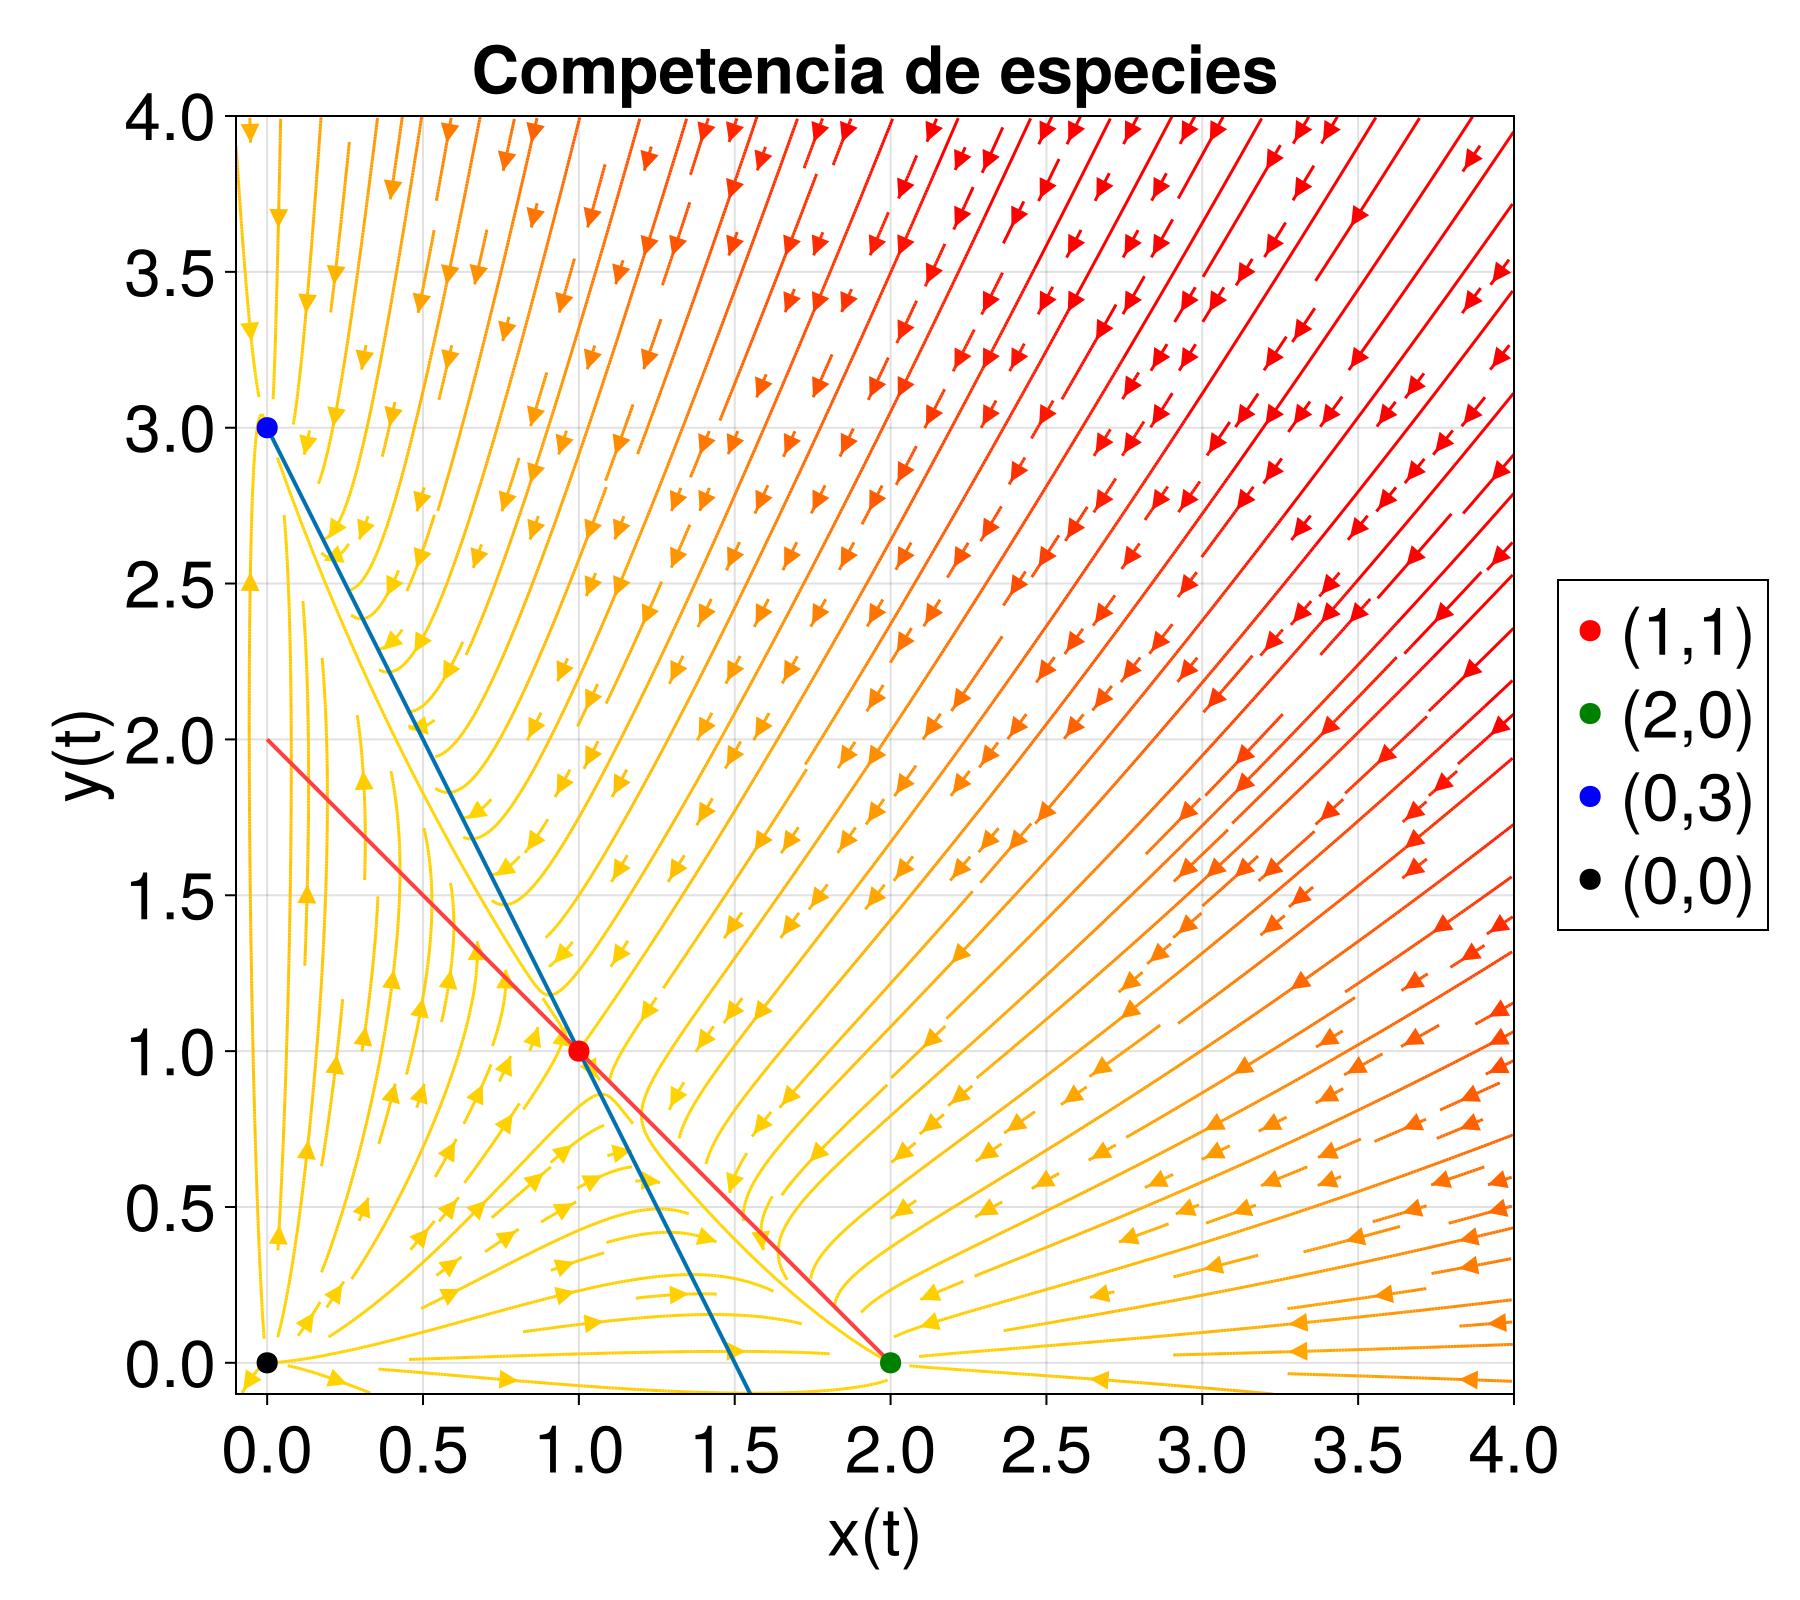
\includegraphics[width=0.5\textwidth]{../Imagenes/Competencia de especies} 
	\end{center} 
	\vspace{-20pt} 
	\caption{Campo vectorial de las soluciones del sistema propuesto de dos especies.} 
	\vspace{-10pt}
	\label{fig:CompetenciaEspecies}
\end{wrapfigure} 
\setlength{\parindent}{0cm}Una vez determinando el espacio fase del sistema, podemos comprobar la estabilidad de los puntos fijos antes encontrados, de tal modo que todas las posibles soluciones terminan convergiendo a uno de los dos atractores posibles. Además de ello podemos observar las dos isoclinas del sistema que no son más que el conjunto de puntos donde se satisface:
\begin{equation*}
	\dot{x}=f(x,y)=0,\qquad\dot{y}=g(x,y)=0
\end{equation*}
a lo largo de la isoclina de $x$ la componente en $x$ es cero y sus soluciones únicamente apuntarán hacia arriba o hacia abajo, dependiendo de la zona. De modo similar ocurre para la isoclina de $y$, en donde la componente $y$ es cero y sus sus soluciones a lo largo de la recta solo pueden ir hacia la derecha o izquierda de forma horizontal. Nuevamente podemos apreciar al punto silla como inestable ya que posicionados ahí y ante una mínima perturbación, el sistema se alejará de este punto e irá convergiendo a cualquiera de los dos atractores (dependiendo de la perturbación). Por último es bien sabido que del origen todas las soluciones divergen debido a la tasa de crecimiento que genera un aumento natural en las poblaciones.\\
\\
%%%%%%%%%%%%%%%%%%%%%CHECKPOINT
%% Nada más checar la aseveración de las isoclinas para ver si se queda o se retira del párrafo
Al tratarse de un sistema simple de dos ecuaciones, se tiene la fortuna poder contar con el espacio fase que nos brinda información crucial sobre su estabilidad, pero ¿Qué ocurre cuando tenemos un sistema de más de 3 especies? como se ha mencionado, la representación visual ya no esta disponible porque cada eje del espacio fase representa a una de las especies que intervienen. A lo mucho podemos acceder a sub-espacios del hiper-espacio fase pero además de que sería engorrosa la generación de cada gráfica, al final solo obtendríamos información a nivel local. 
\\
\\
Si el número de ecuaciones del sistema (\ref{eqn:LK}) llega a ser considerablemente alto, conviene mejor ejecutar una técnica analítica para poder conocer la estabilidad de cada uno de los puntos fijos del sistema, a dicha técnica se le conoce como \textit{linealización}\footnote{agregar referencia}. Particularmente para nuestro sistema, el proceso consiste en bajar el grado de las ecuaciones no lineales para convertirlo a un sistema lineal, y poder operar como se hizo en el capítulo anterior. Los términos no lineales de nuestro sistema (\ref{eqn:LK}) son cuadráticos y basta con bajarles su grado por medio de derivadas parciales. Por lo tanto el proceso de linealización consiste en convertir el sistema (\ref{eqn:LK}) en un sistema lineal aplicándole el \textit{jacobiano}.
\newpage
\begin{definición}
	Sea la función vectorial $\mathbf{F}:\mathbb{R}^n\to\mathbb{R}^n$, entonces el sistema de Lotka-Volterra de especies en competencia se define en su forma vectorial del la siguiente manera
	\begin{equation}\label{eqn:Fmatricial}
		\mathbf{F}(\vec{x})=\begin{pmatrix}
			f_1(\vec{x})\\
			\vdots\\
			f_n(\vec{x}))
		\end{pmatrix},\qquad\text{donde $\vec{x}(t)=\left(x_1(t),...,x_n(t))\right)\in\mathbb{R}^n$.}
	\end{equation}
	donde cada una de las componentes de $\mathbf{F}(\vec{x})$ corresponde con las funciones del sistema (\ref{eqn:LK}), mientras que las componentes del vector $\vec{x}$ corresponden con las especies involucradas. Por lo tanto el sistema (\ref{eqn:LK}) puede ser re-escrito de la siguiente forma
	\begin{equation}\label{eqn:LKmatricial}
		\dot{X}(t) = \mathbf{F}(X(t)),\qquad\text{considerando $\dot{X}(t)=\frac{d\vec{x}(t)}{dt}$}
	\end{equation}
	Nos conviene definir al sistema de esta manera para que podamos ver directamente como se aplica el Jacobiano 
	\begin{equation}\label{eqn:Jacobiano}
		\mathbb{J}_\mathbf{F}(\vec{x}) = \begin{pmatrix}
			\frac{\partial f_1(\vec{x})}{\partial x_1} & \cdots &\frac{\partial f_1(\vec{x})}{\partial x_n}\\
			\vdots & \ddots & \vdots\\
			\frac{\partial f_n(\vec{x})}{\partial x_1} & \cdots &\frac{\partial f_n(\vec{x})}{\partial x_n}
		\end{pmatrix}
	\end{equation}
	El jacobiano resultante al ser evaluado en los puntos fijos del sistema es ahora un sistema lineal al que le podemos extraer sus eigenvalores para poder conocer su estabilidad. Esta matriz es conocida como \textit{matriz de interacciones} ya que guarda en ella la información necesaria para determinar la estabilidad de los puntos fijos del sistema. Sin embargo esta información también se esta limitada a nivel local, pues no será posible que nos brinde información de algún  otro punto fijo.
\end{definición}

\setlength{\parindent}{0cm}Para validar esta aseveración continuaremos con nuestro ejemplo y determinaremos la estabilidad de cada uno de los puntos fijos relacionándolos con lo mostrado en el espacio fase. Para ello aplicamos el jacobiano al sistema de ecuaciones quedándonos con:
\begin{equation}\label{eqn:Jacobiano2}
	\mathbb{J}_\mathbf{F}(\vec{x})=\begin{pmatrix}
		r_1-\frac{2r_1x_1+r_1a_{12}x_2}{K_1} & -\frac{r_1a_{12}x_1}{K_1}\\
		-\frac{r_2a_{21}x_2}{K_2} & r_2-\frac{2r_2x_2+r_2a_{21}x_1}{K_2}
	\end{pmatrix}
\end{equation}
debido a la matriz de incidencias (\ref{eqn:mIncidencias}), se tiene que los valores de la diagonal son $a_{ii}=1$ y corresponden con las auto-interacciones del sistema. Sustituyendo y operando sobre nuestro sistema, al evaluar los puntos fijos antes encontrados se tienen las siguientes matrices de interacciones:
$$
\mathbb{J}_{(2,0)} = \begin{pmatrix}
	-2 & -2\\
	0 & -1
\end{pmatrix},\qquad \mathbb{J}_{(0,3)}=\begin{pmatrix}
	-1 & 0\\
	-6 & -3
\end{pmatrix},\qquad \mathbb{J}_{(1,1)}=\begin{pmatrix}
	-1 & -1\\
	-2 & -1
\end{pmatrix},\qquad \mathbb{J}_{(0,0)}=\begin{pmatrix}
	2 & 0 \\
	0 & 3
\end{pmatrix}
$$
%%%%%%%%Checkpoint
Como previamente se ha revisado, los eigenvalores determinan la estabilidad de un sistema lineal. Se establece que mientras ellos tengan parte real negativa se asegurará que el punto fijo será estable y que en otro caso será inestable. Por lo tanto los eigenvalores de las primeras dos matrices de interacciones deben ser negativos para que sustenten los atractores de la figura (\ref{fig:CompetenciaEspecies}). Mientras que los eigenvalores de $\mathbb{J}_{(1,1)}$ deben ser uno negativo y otro positivo para sustentar al punto silla. Para el caso de la matriz $\mathbb{J}_{(0,0)}$ sus eigenvalores deben tener parte real positiva para que sustenten el repulsor. Realizando el álgebra correspondiente se encuentra lo siguiente
\begin{align*}
	\mathbb{J}_{(2,0)}&\Longrightarrow\ \lambda_1 = -2,\quad\lambda_2 = -1\\
	\mathbb{J}_{(0,3)}&\Longrightarrow\ \lambda_1 = -3,\quad\lambda_2 = -1\\
	\mathbb{J}_{(1,1)}&\Longrightarrow\ \lambda_1 = -1+\sqrt{2},\quad\lambda_2 = -1-\sqrt{2}\\
	\mathbb{J}_{(0,0)}&\Longrightarrow\ \lambda_1 = 2,\quad\lambda_2 = 3\\
\end{align*}
Por tanto se termina de validar la consistencia del método de la linealización al menos para este caso particular. Esta técnica resulta muy útil para obtener la estabilidad de los puntos fijos de forma analítica sin tener que recurrir a una representación visual y como bien se ha mencionado, sobre todo para cuando tengamos sistemas $N$ ecuaciones diferenciales en donde los espacios fase ya son $N$-dimensionales. En la siguiente sección se estará generalizando todo lo mencionado hasta ahora para cuando se tenga dicho escenario.

%%%%%%%%% Checkpoint
\section{Generalizando a N especies}

En la sección anterior se ha introducido el sistema de especies en competencia (\ref{eqn:LK}) y se ha definido su forma vectorial (\ref{eqn:LKmatricial}) generalizada; se mostró un ejemplo particular con $n=2$ para observar su dinámica a través de su espacio fase (figura (\ref{fig:CompetenciaEspecies})) en donde se contempla la naturaleza de sus puntos fijos si se trata de atractores, repulsores o puntos silla. Se propone el método de la linealización para conseguir matrices de interacción que determinen de forma analítica la estabilidad de cada uno de los puntos fijos del sistema. En esta sección se profundizará más acerca de lo mencionado comenzando con la construcción matriz de incidencias que será eje fundamental de las interacciones del sistema de $N$ especies. \\
\\
Hasta ahora se ha estado discutiendo puramente sobre dinámica y ecuaciones diferenciales, sin embargo, el lector recordará al principio del primer capítulo que se ha mencionado sobre el uso estratégico de redes para poder modelar cierto sistema dinámico no lineal, en este caso para representar las interacciones de (\ref{eqn:LK}): por lo tanto, ahora toca hablar un poco sobre redes. Una red es considerada una colección de \textit{nodos} que se encuentran unidos por \textit{enlaces}\footnote{definir más adelante el tipo de interacciones con base en el signo y si son dirigidas o no dirigidas. Además de agregar cita del Newman para esta definición.}. Para definir redes siempre es necesario establecer que es lo que representan los nodos y que representan los enlaces, en nuestro caso los nodos representan directamente las especies que participan en el sistema mientras que los enlaces serían sus interacciones, más adelante veremos su naturaleza.\\
\\
Si definimos un conjunto de especies $x_i$ y sabemos que se relacionan por medio de los coeficientes $\alpha_{ij}$ de 
\begin{wrapfigure}{l}{0.45 \textwidth} \vspace{-30pt} \begin{center}
		\includesvg[width=.5\textwidth]{../Imagenes/karateLu} 
	\end{center} 
	\vspace{-20pt} 
	\caption{Red de Karate de Zachary} 
	\vspace{-20pt}
	\label{fig:RedKarate}
\end{wrapfigure} 
(\ref{eqn:LK}), entonces decimos que una interacción entre las especies $x_i$ y $x_j$ (nodos de la red) es para cuando $\alpha_{ij}\neq 0$ y esto representaría un enlace en la red. En el mundo es posible encontrar diferentes tipos de redes con cierto significado, tales como la red de energética de un país, redes de amistades en una universidad o redes de acciones que cotizan en la bolsa de valores; en el caso de la Figura (\ref{fig:RedKarate}) es una red conocida por quienes se dedican a ello y es la representación de una red social llamada \href{https://en.wikipedia.org/wiki/Zachary%27s_karate_club}{Red del club Karate de Zachary}. Para poder representar estas redes y cualquier otro tipo de red conviene introducir el concepto de \textit{matriz de adyacencia.}
\begin{definición}\label{def:matrizdeadyacencia}
	Sea $A\in\mathcal{M}_n(\mathbb{R}) $. Se define la matriz de adyacencia tal que sus entradas son de la siguiente forma
	$$a_{ij}= 
	\begin{cases}
		1, \ \text{si $\exists$ un enlace entre el nodo $i$ y el nodo $j$.}\\
		0, \ \text{en otro caso}.
	\end{cases}$$
	La matriz de adyacencia será la herramienta para determinar la relación de interacción entre especies, pero solo hablará de su existencia y se tendrán que agregar algunas características para darle los pesos de interacción, mismos que están representados por los coeficientes $\alpha_{ij}$ del sistema (\ref{eqn:LK}) 
\end{definición}
%%%%%%% Checkpoint
\begin{ejemplo}
	Para poder apreciar la matriz de adyacencia definamos una red de 10 nodos y veamos la matriz de adyacencia que le corresponde. Cada nodo ha sido marcado para poderlo identificar y relacionar con la matriz de adyacencia. Los renglones y columnas de la matriz representan los nodos, siendo el primer renglón el primer nodo (número 1), el quinto renglón será el quinto nodo (número 5); esto pasa de manera equivalente con las columnas, la cuarta columna corresponde con el cuarto nodo (número 4), la octava columna corresponde con el octavo nodo (número 8). Por tanto, mediante la matriz de adyacencia sabemos que el primer nodo (renglón 1) esta enlazado con el noveno nodo (columna 9) ya que existe un uno, mientras que el primer renglón y la quinta columna hay un cero lo que indica que no existe un enlace entre estos nodos. 
\end{ejemplo}
\begin{wrapfigure}{r}{0.5 \textwidth} \vspace{-30pt} \begin{center}
		\includesvg[width=0.5\textwidth]{../Imagenes/red10Lu} 
	\end{center} 
	\vspace{-20pt} 
	\caption{Red no dirigida de 10 nodos.} 
	\vspace{-150pt}
	\label{fig:Red10}
\end{wrapfigure} 

$$
A=\begin{pmatrix}
	0 & 1 & 0 & 1 & 0 & 0 & 0 & 0 & 1 & 0 \\
	1 & 0 & 1 & 0 & 0 & 1 & 0 & 0 & 0 & 0 \\
	0 & 1 & 0 & 0 & 0 & 0 & 1 & 1 & 0 & 0 \\
	1 & 0 & 0 & 0 & 1 & 1 & 1 & 0 & 0 & 1 \\
	0 & 0 & 0 & 1 & 0 & 0 & 0 & 0 & 1 & 1 \\
	0 & 1 & 0 & 1 & 0 & 0 & 1 & 1 & 0 & 1 \\
	0 & 0 & 1 & 1 & 0 & 1 & 0 & 0 & 1 & 0 \\
	0 & 0 & 1 & 0 & 0 & 1 & 0 & 0 & 1 & 0 \\
	1 & 0 & 0 & 0 & 1 & 0 & 1 & 1 & 0 & 1 \\
	0 & 0 & 0 & 1 & 1 & 1 & 0 & 0 & 1 & 0 \\
\end{pmatrix}
$$
También hay que destacar qué la matriz es simétrica y que la diagonal es igual a cero: para el primer punto se debe notar que la relación de los enlaces entre nodos no tiene dirección, es decir, que exista un enlace entre nodos significa que el nodo $i$ se conecta con $j$ y viceversa, que el nodo $j$ se conecta con el nodo $i$. Por tanto decimos que la red de la figura (\ref{fig:Red10}) es \textit{no dirigida} puesto que no hay una dirección preferencial en el enlace. Para el segundo punto se puede deducir que los nodos podrían relacionarse consigo mismo, en este caso caso particular no lo hacen pero si es posible la existencia de \textit{autoenlaces}. Para el sistema (\ref{eqn:LK}) los autoenlaces representan las autointeracciones que dan el caracter logístico de las ecuaciones. En cuanto se defina la matriz de interacciones se verá el papel que toman los elementos de la diagonal y de porque deben de existir autoenlaces en cada una de las ecuaciones del sistema.	
\\
\\
Cuando se tiene el caso en que los enlaces tienen una dirección preferencial de nodo a nodo, decimos que corresponde a una \textit{red dirigida}. En este caso el enlace podrá ir del nodo $i$ al nodo $j$ pero no necesariamente lo hará en sentido contrario, deberá definirse explícitamente. En el mundo también existe un gran conjunto de redes dirigidas como lo son las citaciones académicas, la propia WWW (World Wide Web), incluso redes tróficas de depredador-presa. Y para este caso también se tiene asociada una matriz de adyacencia con una ligera diferencia con respecto de la definición \ref{def:matrizdeadyacencia}.
\begin{definición}
	Sea $D\in\mathcal{M}_n(\mathbb{R})$, matriz de adyacencia de una red no dirigida. Se definen sus elementos de la siguiente manera:
	$$
	\alpha_{ij}=\begin{cases}
		1,\qquad\text{Si existe un enlace del nodo $i$ al nodo $j$}\\
		0,\qquad\text{otro caso.}
	\end{cases}
	$$
	Los enlaces de las redes dirigidas van a estar representados por flechas para que puedan mostrar adecuadamente las direcciones correspondientes entre los nodos. 
\end{definición}

\begin{ejemplo}
	Se tiene la siguiente red dirigida de 10 nodos con exactamente 14 enlaces. La matriz de adyacencia asociada es la siguiente
\end{ejemplo}

\begin{wrapfigure}{l}{0.5 \textwidth} \vspace{-30pt} \begin{center}
		\includesvg[width=0.52\textwidth]{../Imagenes/Red10DirLu} 
	\end{center} 
	\vspace{-20pt} 
	\caption{Red no dirigida de 10 nodos.} 
	\vspace{-150pt}
	\label{fig:Red10Dir}
\end{wrapfigure} 
$$
D = \begin{pmatrix}
	0 & 0 & 0 & 0 & 0 & 0 & 0 & 0 & 0 & 1 \\
	1 & 0 & 1 & 0 & 0 & 0 & 0 & 1 & 0 & 0 \\
	0 & 0 & 0 & 1 & 1 & 0 & 0 & 0 & 0 & 1 \\
	1 & 0 & 0 & 0 & 0 & 0 & 0 & 0 & 0 & 0 \\
	0 & 0 & 1 & 0 & 0 & 0 & 0 & 1 & 0 & 0 \\
	0 & 1 & 0 & 0 & 0 & 0 & 0 & 0 & 0 & 0 \\
	0 & 0 & 1 & 0 & 0 & 0 & 0 & 0 & 0 & 0 \\
	0 & 0 & 0 & 0 & 0 & 0 & 0 & 0 & 0 & 0 \\
	0 & 1 & 0 & 0 & 0 & 0 & 0 & 0 & 0 & 0 \\
	0 & 0 & 0 & 0 & 0 & 0 & 1 & 0 & 0 & 0 \\
\end{pmatrix}
$$

Ahora se puede notar que la matriz de adyacencia no es simétrica y que por lo tanto los enlaces presentan una dirección preferencial. Ambas visiones se van a tomar en cuenta para modelar al sistema de especies en competencia, sin embargo, preferentemente tendrá mayor protagonismo la \textit{red no dirigida} que la otra ya que como se verá más adelante, producen los mismos resultados y la diferencia recae en el tiempo de obtención de los datos en donde las redes dirigidas requieren mayor tiempo de compilación para generar escenarios estables.\\
\\
En este punto el lector ya debe suponer la razón de la presentación de estas dos formas de redes; el sistema dinámico de especies en competencia considera las interacciones dadas por los coeficientes $\alpha_{ij}$, sin embargo puede que exista el coeficiente $\alpha_{ij}$ que relaciona a la especie $x_i$ con la $x_j$ pero bien podría suceder que $\alpha_{ji}=0$ y en consecuencia no exista interacción de la especie $x_j$ con la especie $x_i$. Por lo tanto la matriz de incidencias, esta construida con base en alguna de estas dos formas de red. 

\subsection{Red de incidencias}

La \textit{red de incidencias} es el artilugio principal que se va a ocupar para poder modelar las interacciones del sistema de especies en competencia, tiene asociada una matriz de adyacencia que llamaremos \textit{matriz de incidencias} y se va a componer de tres factores: puede ser de una red dirigida o no dirigida, las interacciones son importantes y definir la dirección de las mismas hace más completo al sistema, sin embargo usaremos mayormente redes no dirigidas. La topología de la red que se va a utilizar es la conocida \textit{red aleatoria} de Erdös–Rényi [Cita\footnote{poner cita de esto}] que nos van a modelar interacciones entre las especies de forma aleatoria con base en cierto parámetro. Y aunado a todo ello tendremos una matriz de pesos en donde sus entradas se encuentran en una distribución normal centrada en el cero. La conjunción de estos tres elementos da lugar a la matriz de incidencias y por lo tanto a su red asociada.\\
\\
La red de Erdös–Rényi es ampliamente utilizada aprender sobre estructura y propiedades de la redes y poder utilizar ese conocimiento para aplicarlo a las llamadas \textit{redes libres de escala}. La diferencia sustancial entre la red aleatoria y la red libre de escala es que la primera tiene muy pocas (o ninguna) aplicaciones en escenarios de la naturaleza, se ha encontrado que las estructuras de las redes en la naturaleza siguen cierto patrón y distribución que se han englobado en las redes libres de escala. Sin embargo en este trabajo únicamente veremos que información nos brinda aplicar el modelo de Erdös–Rényi al sistema (\ref{eqn:LK}) con la intención de extender el trabajo a redes libres de escala\footnote{Un modelo teórico que rescata todas las propiedades de las redes libres de escala es el de Albert-Barabasi [Cita].}. 
\begin{definición}\label{def:redAleatoria}
	Sean un conjunto de $N$ nodos sin enlaces asociados. Para cada par de nodos $i$ y $j$ de las $\binom{N}{2}$ posibles combinaciones se definen sus enlaces aleatorios dada una probabilidad $p$ y un número aleatorio $r$ en el intervalo $[0,1]$ de la siguiente forma
	$$
	L_{ij}=\begin{cases}
		\exists,\qquad\text{Si }r<p\\
		\nexists,\qquad\text{Si }r\geq p
	\end{cases}
	$$
	El conjunto de los $N$ nodos con sus posibles $L_{ij}$ enlaces forman la red aleatoria de Erdös–Rényi. En esta referencia [cita\footnote{referencia a barabasi}] el lector podrá conocer más sobre las propiedades de esta red, nosotros por ahora solo la ocuparemos sin enfocarnos en sus propiedades. La matriz de adyacencia de esta red aleatoria es simétrica lo que nos da entender que la red es no dirigida en esencia. Podemos extender esta definición a redes aleatorias dirigidas suponiendo que la conexión va en dirección del nodo $i$ al nodo $j$ y considerar también conexiones del nodo $j$ al nodo $i$, por lo tanto ahora tendremos $N(N-1)$ posibles combinaciones de nodos. \\
	\\
	Si solo se considerara uno de los dos casos, es decir, para $\binom{N}{2}$ combinaciones de nodos entonces tendríamos la mitad de posibles conexiones, la matriz de adyacencia sería triangular superior por haber considerado únicamente la dirección de $i$ a $j$. Para llenar la parte triangular inferior de esta matriz debemos considerar las conexiones de $j$ a $i$ y haciéndolo habremos obtenido nuestra red aleatoria dirigida. En la sección (\ref{sec:RedesAleatorias}) se encuentra la implementación computacional de ambas visiones de la red aleatoria.
\end{definición}
\newpage
\setlength{\parindent}{0cm}En este punto estamos a un solo paso de construir finalmente a la matriz de incidencias, únicamente nos falta de considerar la magnitud de las interacciones entre especies y para ello se va a emplear una matriz de $N\times N$ donde $N$ es el número de nodos de la red que vayamos a modelar; esta matriz se va a mapear con una función de densidad de probabilidad (FDP) asociada a una distribución normal en cada entrada
$$f(x)=\frac{1}{\sigma\sqrt{2\pi}}e^{-\frac{(x-\mu)^2}{2\sigma^2}}$$
en esencia será una matriz con entradas aleatorias bajo una FDP centrada en $\mu = 0$ y variando a sigma en $[0,1]$ con un paso de $0.1$ (esto se irá detallando más adelante). 
\begin{definición}
	Sea una red aleatoria de $N$ nodos dirigida o no dirigida y $A$ su matriz de adayacencia asociada, definimos así mismo una matriz de entradas aleatorias $M$ mapeada bajo una FDP centrada en $\mu=0$ y con $\sigma\in[0,1]$. Definimos a $\Lambda$ la \textit{matriz de incidencias} como el producto de Hadamard (entrada a entrada) de la matriz de adyacencia con la matriz aleatoria sumada con la matriz identidad:
	$$\Lambda=(A\odot M) + I$$
	El producto $A\odot M$ simplemente agrega pesos a cada posible enlace de a la matriz de adyacencia asociada a la red aleatoria, y seguida la suma con la identidad es para poder agregar autoenlaces a cada nodo de la red aleatoria.
\end{definición}
\setlength{\parindent}{0cm}Esta matriz tendrá inmersa una topología de red aleatoria cuyos enlaces tienen pesos y en donde forzamos los autoenlaces en cada uno de los nodos con un peso $w=1.0$. Por lo tanto es posible definir una 
\begin{wrapfigure}{r}{0.5 \textwidth} \vspace{-30pt} \begin{center}
		\includesvg[width=0.52\textwidth]{../Imagenes/RedIncidencias} 
	\end{center} 
	\vspace{-20pt} 
	\caption{Red de incidencias de 8 nodos bajo la topología de una red aleatoria dirigida con $p=0.15$ y una matriz aleatoria con $\mu=0$ y $\sigma=0.2$.} 
	\vspace{-10pt}
	\label{fig:RedIncidencias}
\end{wrapfigure} 
\textit{red de incidencias} en donde cada enlace tendrá un peso asociado. En embargo, por la forma en como consideramos $M$, red de incidencias resultante es forzosamente dirigida, independientemente de la elección de red aleatoria. Hablando específicamente para el caso en donde se considera $A$ simétrica (red no dirigida), al momento de realizar el producto punto con $M$, las entradas $\alpha_{ij}$ no necesariamente son iguales a su parte simétrica, por lo que se tendrá un peso para el enlace $i\to j$ y otro peso para el enlace $j\to i$. Si la matriz aleatoria $M$ tuviera entradas aleatorias en la parte triangular superior y simetrizáremos hacia la parte triangular inferior, entonces así tendríamos una red de incidencias no dirigida con $\Lambda$ enterametne simétrica.

\newpage
Relacionando los coeficientes del sistema con las formas de red que tenemos hasta ahora, queda preguntarnos sobre las implicaciones de que $\alpha_{ij}\in\mathbb{R}$, ¿para todo valor posible de $\alpha_{ij}$ se tendrá un comportamiento homogéneo o será acaso que tendremos escenarios particulares? May nos brinda la respuesta [cita\footnote{poner cita  del libro de ecología.}] con un abanico de 5 posibles escenarios. Antes de presentar los escenarios hay que resaltar el hecho de que el signo de $\alpha_{ij}$ importa mucho más que el propio valor (peso) que se le asigne, ya que tiene repercusiones en la ecuación (\ref{eqn:LK}) en donde los elementos de la suma dentro del paréntesis están siendo afectados por el signo negativo que posee a su izquierda; particularmente si tenemos $\alpha_{ij}<0$ entonces la relación de la especie $x_i$ con la $x_j$ ya no se va a restar sino a sumar y eso impacta significativamente en la dinámica del sistema, esto se irá viendo más adelante.\\
\\
May establece que tenemos 5 posibles interacciones repartidas de la siguiente forma: para la red no dirigida únicamente podemos acceder a dos tipos de interacciones las de competencia $(--)$ y las de mutualismo o simbiosis\footnote{A mi me gusta llamarles de cooperación, así que de ahora en adelante de esa forma me estaré refiriendo a ellas.} $(++)$. La matriz de adyacencia de una red no dirigida al ser simétrica, sus coeficientes cumplen $A_{ij}=A_{ji}$ por lo que en principio tendrán mismo signo aunque podrían tener diferentes pesos, cuando sus signos son positivos implica que la especie $x_i$ y la especie $x_j$ se encuentran en una relación de competencia por lo que dependiendo de los pesos (y claro que de las condiciones iniciales) una de las dos especies intentará sobreponerse sobre la otra. En el caso en donde los signos de las entradas simétricas de la matriz de adyacencia son negativos, ocurre el caso contrario, la especie $x_i$ coopera con la especie $x_j$ y fomentan sus crecimientos gracias a ello, la forma de su cooperación también va a depender de los pesos que les sean asignados.\\
\\
Para el caso de la red dirigida pueden acceder a los 5 tipos de interacción ya que bien pueden existir entradas simétricas aunque la matriz en general no lo sea, las que nos faltan son: el comensalismo (+0)


